Image classification has been around for many years now. Still, as a subpart of computer vision, it is nowadays one topic of high interest, due to the increasing number of images available on the web and the amount of information we can obtain from them.  Therefore, we have chosen to apply SVM techniques to Image classification problem, to both gain experience in applying SVM to a practical real-life problem, and at the same time, to get some idea of the main challenges of computer vision. 
Images of $N\times M$ pixels, each pixel belonging to $[0..255]$ or $[0..1]$, can be represented as a vector $x \in \mathbb{R}^{N\cdot M}$. Then, any classifier we use will take this vector as input for each image. The problem of this representation for images is that images that are very similar to the human eye, can be treated as very different when measured by a pixel-wise distance measure like the Euclidean norm (See Figure[\ref{fig:handwrite}]).  The reason for this is that that pixel-wise representation lacks of invariance with respect to some transformations that human eye is able to detect as similar. Some of these transformation include translations, (small) rotations, (small) changes in size, blur, brightness and contrast (See Figure[\ref{fig:handwriteinvar}]) are factors that humans typically consider irrelevant when judging if two images show the same object. 
\begin{figure}[!h]
    \centering
    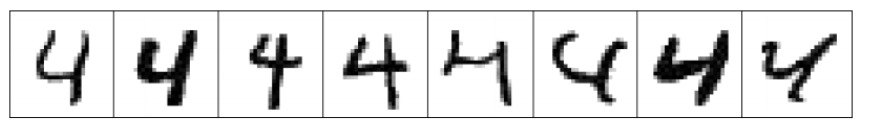
\includegraphics[width=0.9\textwidth]{Images/handwrite4.jpg}
    \caption{Handwritten digit 4 - different appearances}
    \label{fig:handwrite}
\end{figure}
\begin{figure}[!h]
    \centering
    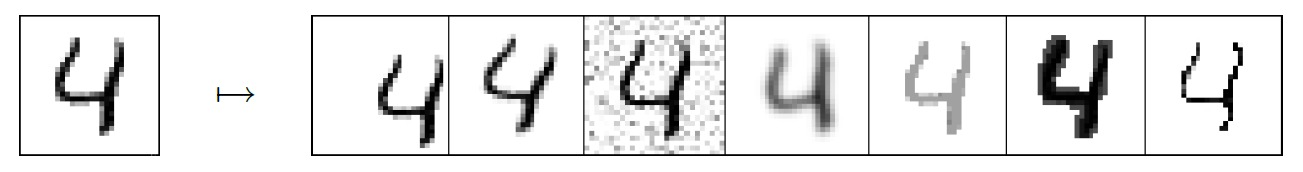
\includegraphics[width=0.9\textwidth]{Images/handwrite4transformations.jpg}
    \caption{Handwritten digit 4 - different transformations}
    \label{fig:handwriteinvar}
\end{figure}
How to deal with this variance in images has been extensively studied in computer vision field. Mainly, there are four options to deal with it. 
\begin{itemize}
    \item Extending the training set. 
    \item Normalization of the image. 
    \item Integrating invariance in the kernel. 
    \item Finding invariant features representations. 
\end{itemize}

The most widely developed and effective approach so far has been to find invariant features representation. In our project, we will combine two invariant representations: the gradient representation and the histogram representation. Combined, they are what is called Histogram of Gradients representation in Computer Vision literature. These two representations will be explained more in depth in the \textit{Theory section}[\ref{section:theory}]. Depending on the granularity at which histograms of gradients are obtained, more grained or less grained representations of the image can be obtained (See Figure[\ref{fig:hog_levels}]). So, one of the points we will study is which is the optimal representation of the image in terms level of granularity at which histograms of gradients will be computed. 

\begin{figure}[!h]
    \centering
    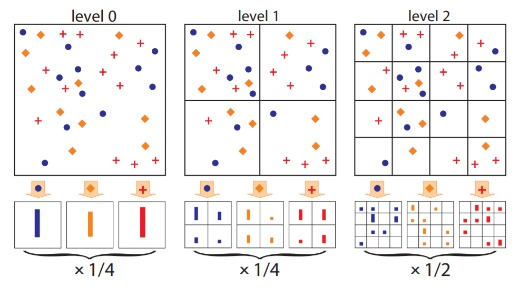
\includegraphics[width=0.9\textwidth]{Images/hog_levels.jpg}
    \caption{Example of constructing a pyramid for L = 2}
    \label{fig:hog_levels}
\end{figure}

On the other side, we want to test the capability of SVM to fit and generalize the feature invariant representations that we have obtained with the histograms of gradients. For this we will try the generalization performance of several different kernels such as the linear kernel or the RBF kernel. We will run several experiments and try to explain why some kernels generalize better depending on the chosen HOG representations. For instance, we may find that for representations with HOG obtained at level 0 of the image (See Figure[\ref{fig:hog_levels}]), the radial kernel outperforms the others, while for representations with HOG obtained at level 2, the linear kernel outperform the others.

As for the dataset, we have chosen the \textbf{Caltech 101} images dataset that contains images classified in 101 categories, each category having different number of images. In order to avoid problems derived from imbalanced datasets, we have decided to to keep only the categories that have 70 or plus images, resulting in 31 categories. For the purpose of interpretability of results, this may be too much categories. Ideally, we would like to have a smaller subset of categories but that are different in nature, meaning that some of them are hard to classifiy and some are easy. To select categories that meet this criteria, we have launched a classification with a linear SVM and the 31 categories, obtaining the Specificity for each of the categories:

\begin{table}[H]
\centering
\begin{tabular}{|c|c|}
\hline
\textbf{Class}& \textbf{Sensitivity}      \\ \hline
{car\_side}        & {1}    \\ \hline
{trilobite}        & {1}    \\ \hline
{airplanes}        & {0.95} \\ \hline
{minaret}          & {0.95} \\ \hline
{ketch}            & {0.9}  \\ \hline
{Motorbikes}       & {0.9}  \\ \hline
{Faces}            & {0.8}  \\ \hline
{grand\_piano}     & {0.75} \\ \hline
{helicopter}       & {0.75} \\ \hline
{Leopards}         & {0.75} \\ \hline
{revolver}         & {0.7}  \\ \hline
{chandelier}       & {0.65} \\ \hline
{ewer}             & {0.65} \\ \hline
{laptop}           & {0.65} \\ \hline
{watch}            & {0.65} \\ \hline
\end{tabular}
\centering
\begin{tabular}{|c|c|}
\hline
\textbf{Class}& \textbf{Sensitivity}      \\ \hline
{bonsai}           & {0.6}  \\ \hline
{electric\_guitar} & {0.6}  \\ \hline
{menorah}          & {0.6}  \\ \hline
{sunflower}        & {0.6}  \\ \hline
{umbrella}         & {0.6}  \\ \hline
{brain}            & {0.55} \\ \hline
{buddha}           & {0.55} \\ \hline
{butterfly}        & {0.55} \\ \hline
{crab}             & {0.55} \\ \hline
{kangaroo}         & {0.55} \\ \hline
{llama}            & {0.55} \\ \hline
{hawksbill}        & {0.5}  \\ \hline
{ibis}             & {0.45} \\ \hline
{scorpion}         & {0.3}  \\ \hline
{starfish}         & {0.3}   \\ \hline
\end{tabular}
\end{table}

So, we have selected some "easy" categories, some "medium" and some "hard", up to 10. The chosen ones will be: scorpion, starfish, airplanes, bonsai, faces, minaret, motorbikes, trilobite, umbrella, watch. So this results in 10 classes, with 70 images per class. 
